\documentclass{article}

\usepackage{caption}

\usepackage{multirow}

\usepackage{graphicx}
\setlength{\abovecaptionskip}{10pt plus 3pt minus 2pt}
\setlength{\belowcaptionskip}{10pt plus 3pt minus 2pt}

\usepackage[margin=1in]{geometry}

\usepackage{hyperref}
\hypersetup{
    pdfborderstyle={/S/U/W 1},
    colorlinks=true,
    linkcolor=blue,
    filecolor=magenta,
    urlcolor=cyan,
}

\usepackage{algorithm,algpseudocode}

\usepackage{xcolor}
\usepackage{listings}
\lstdefinestyle{DOS}{
    backgroundcolor=\color{lightgray},
    basicstyle=\scriptsize\color{black}\ttfamily
}

\title{\vspace{-2em}
CSE 5441 (Fall 2019, Dr. Jones)\\
\large \texttt{CUDA} (Lab 4)
}
\author{
Caleb Lehman \\
\href{mailto:lehman.346@osu.edu}{lehman.346@osu.edu}
}

\begin{document}
\maketitle

\section*{Overview}
\label{sec:overview}

For this lab, I parallelized my serial \texttt{C} program to perform Adaptive Mesh
Refinement (AMR)\footnote{See lab 1 or project descriptions for details about
AMR computation.} using the \texttt{CUDA} API. I created 2 programs,
\texttt{cuda-disposable} and \texttt{cuda-persistent}, which mirror the
disposable and persistent threads models used in the previous labs. In
particular, the \texttt{disposable} code runs a new kernel for each iteration,
while the \texttt{persistent} code has a single kernel which synchronizes the
threads between iterations\footnote{Because the \texttt{CUDA} API doesn't directly provide a simple way
to synchronize blocks, the \texttt{cuda-persistent} version is limited to running with a single block of
threads.}.

\section*{Tests}
\label{sec:tests}

\subsection*{Environment}
\label{subsec:environment}

The program was developed and tested on the
\href{https://www.osc.edu/resources/technical_support/supercomputers/owens}{Owens
cluster} at the \href{https://www.osc.edu/}{Ohio Supercomputer Center}.  Note
that all my other labs were developed and tested on the
\href{https://www.osc.edu/resources/technical_support/supercomputers/pitzer}{Pitzer
cluster}, which has different specifications.

For development and testing, I loaded the \texttt{cuda/9.2.88} module, which
allowed the program to be compiled with version 9.2.88 of the \texttt{nvcc}
compiler, as well as setting some environment variables pointing to
\texttt{CUDA}-related headers and libraries.

For testing, I loaded the \texttt{python/3.6-conda5.2} module, which loads a
python environment with the \texttt{NumPy}, \texttt{SciPy}, and
\texttt{Matplotlib} packages, amoung others. \texttt{Python} is only necessary
for collecting and plotting the data from testing, not for the actual exectuion
of the program.

\subsection*{Timing}
\label{subsec:timing}

I collected timing data using the same 4 methods as the first several labs:
\texttt{time}, \texttt{clock}, and \texttt{clock\textunderscore gettime} from
the \texttt{"time.h"} header, and the \texttt{UNIX} utility \texttt{time}.

As with the second and third labs, I didn't use the results from the \texttt{clock}
function from the \texttt{"time.h"} header, since it reports CPU time, not wall
time. The other methods all returned values within 1 second of each other. The
\texttt{time} function declared in \texttt{"time.h"} returns an integer number
of seconds, but the other two methods return with sub-second precision.
\emph{For consistency, I used the \texttt{clock\textunderscore gettime}
function for all results in this report}.

\subsection*{Test Files}
\label{subsec:test_files}

Dr. Jones provided the \texttt{testgrid\textunderscore 400\textunderscore
12206} test file.  As part of lab 1, I reduced the $\alpha$ (affect rate) and
$\varepsilon$ parameters until the serial runtime increased into the 3 to 6
minute range. In particular, I selected $\alpha = 0.01$ and $\varepsilon =
0.02$, for which the serial program completed in 261 seconds. However, my \texttt{CUDA}
implementations yielded very poor performance, so I ended up using parameters of
$\alpha = 0.1$ and $\varepsilon = 0.1$\footnote{In any case, these parameters really
only affect the final DSV values and number of iterations, not the actual amount of work
done per iteration, so most of the relative results found in this report should be the same
for different values of $\alpha$, $\varepsilon$.}.  For this reason, and due to using the
Owens cluster instead of the Pitzer cluster, it isn't particularly useful to
compare the results from this lab to the results from labs 2 and 3.

\newpage
\section*{Results}
\label{sec:results}

The output was consistent across both programs and was as follows:
\begin{itemize}
    \item \texttt{testgrid\textunderscore 400\textunderscore 12206}: 75197 iterations, $(max, min) = (0.077873, 0.086525)$
\end{itemize}

The relevant runtimes for the serial, \texttt{cuda-persistent}, and \texttt{cuda-disposable}
versions on the test case are visualized in the figures below. I found that the
\texttt{cuda-persistent} version had optimal performance around 320 threads (and 1 block) and
the \texttt{cuda-disposable} version had optimal performance with 32 threads and 10 blocks.
Those values are now hardcoded into the program, as requested.
With the optimal values for threads and blocks,
\texttt{cuda-persistent} ran in 106 seconds and \texttt{cuda-disposable}
ran in 54 seconds.

The two biggest implications I see in this expirement are:
\begin{itemize}
    \item My serial program (with the same $\alpha=0.1, \varepsilon=0.1$
    parameters) runs in 14 seconds, so the \texttt{CUDA} versions are
    significantly slower. Since other parallelization methods (\texttt{OpenMP}
    and \texttt{pthreads}) improved performance, this indicates that my
    \texttt{CUDA} implementation was probably poorly done. I wasn't able to
    determine why the performance was so bad, but I suspect that it has
    something to do with cache performance, since the cache on the GPU is much
    smaller than that on the CPU.

    \item When comparing the \texttt{cuda-persistent} and
    \texttt{cuda-disposable} version with the same thread/block parameters, the
    \texttt{cuda-disposable} version consistently performed better. For
    example, when both programs used 256 threads and 1 block,
    \texttt{cuda-disposable} ran in 110 seconds, while \texttt{cuda-persistent}
    ran in 124 seconds.  This shows that it is faster to kill and restart the
    entire kernel (\texttt{cuda-disposable}) than to just synchronize the
    threads (which do slightly uneven amounts of work in
    \texttt{cuda-persistent}).  This is the opposite of the behaviour I noticed
    in the \texttt{pthreads} lab, confirming that \texttt{CUDA} threads are
    much more lightweight than even the relatively lightweight
    \texttt{pthreads}.
\end{itemize}

\vspace{1em}
\begin{minipage}{\linewidth}
    \begin{minipage}{.4\linewidth}
    \centering
    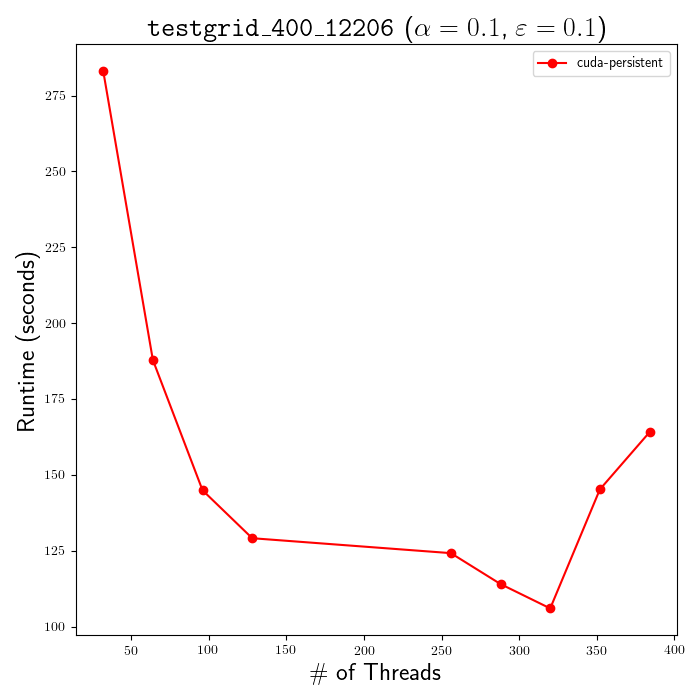
\includegraphics[width=.8\linewidth]{../cuda-persistent.png}
    \end{minipage}
    \hfill
    \begin{minipage}{.5\linewidth}
    \centering
    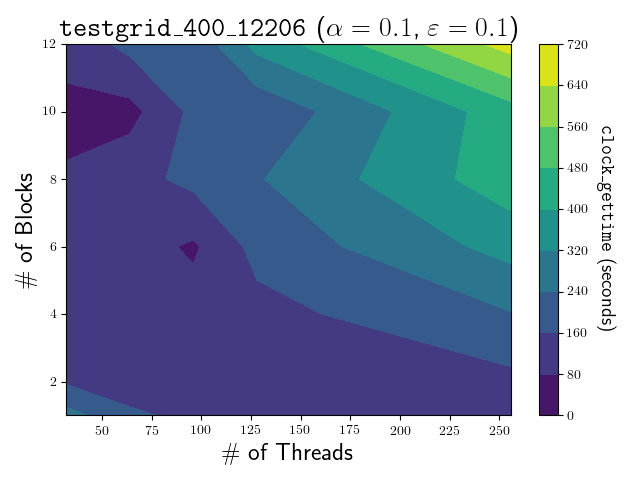
\includegraphics[width=.8\linewidth]{../cuda-disposable.png}
    \end{minipage}
    \captionof{figure}{The runtimes of the \texttt{cuda-persistent} (left)
    and \texttt{cuda-disposable} (right) parallelizations.
    Note that, due to the poor performance
    of the \texttt{CUDA} parallelization, higher $\alpha$ and
    $\varepsilon$ parameters were used compared to previous labs.
    For comparison, my serial program runs in 14 seconds with
    these parameters. \textbf{Important note:} the \texttt{cuda-persistent}
    plot displays the runtimes on a scale starting at 100 seconds.}
\end{minipage}

\pagebreak
The following is the series of computations performed for the $i$th box during each iteration,
which make up basically all of the ``useful'' work done in the programs:

\begin{lstlisting}[style=DOS]
updated_vals[i] = box->self_overlap * current_vals[i];
for (int nhbr = 0; nhbr < box->num_nhbrs; ++nhbr) {
    updated_vals[i] += box->overlaps[nhbr] * current_vals[box->nhbr_ids[nhbr]];
}
updated_vals[i] /= box->perimeter;
updated_vals[i] = current_vals[i] * (1 - affect_rate)
    + updated_vals[i] * affect_rate;
\end{lstlisting}

The number of arithmetic operations in the above sample is $1 + 2 \cdot N_i + 1 + 4$, where
$N_i$ is the number of neighbors of the $i$th box. Letting $n$ be the number of boxes,
$N$ be the total number of neighbors (counted with multiplicities), and $I$ be the number of iterations,
the total number of arithmetic operations is given by $I\cdot (6n + 2N)$. For the given test file
(\texttt{testgrid\textunderscore 400\textunderscore 12206}) and choice of
parameters ($\alpha=0.1, \varepsilon=0.1$), we have the values $I=75197$, $n=12206$, and $N=71890$.
Substituting in these values, I computed $GFlops = \frac{ops / 10^9}{\# of seconds} = \frac{16.32}{\# of seconds}$
for each of the programs to get the following results\footnote{I
used the optimal times from each of the \texttt{CUDA} programs for this computation.}:

\begin{center}
\begin{tabular}{|c|c|c|c|}
\cline{2-4}
\multicolumn{1}{c|}{} & serial & \texttt{cuda-disposable} & \texttt{cuda-persistent} \\
\hline
GFlops & 1.166 & 0.302 & 0.154 \\
\hline
\end{tabular}
\end{center}

\section*{Project Usage}
\label{sec:project}

\subsection*{Building}
\label{subsec:building}

To build the \texttt{cude-disposable} and \texttt{cude-persistent} executables, navigate
to the top level of the submitted directory and build as follows:

\begin{lstlisting}[style=DOS]
# Ensure that you have nvcc compiler

# Note that the provided makefile
# assumes the CUDA_HOME environment
# variable is set appropriately

# On the OSC clusters, this can be achieved
# with the command:
$ module load cuda

$ make
$ ls
... cuda-persistent cuda-disposable ...
\end{lstlisting}

\subsection*{Running}
\label{subsec:running}

The syntax to run the program is:

\begin{lstlisting}[style=DOS]
$ ./[program] [affect-rate] [epsilon] <[test-file]
\end{lstlisting}
where \texttt{program} is one of $\{\texttt{cuda-persistent}, \texttt{cuda-disposable}\}$

\end{document}
